\documentclass[tikz,border=0pt]{standalone}
% Deterministic vector typography; formulas are compiled by XeLaTeX.
\usepackage{fontspec}
\IfFontExistsTF{Comic Sans MS}{\setmainfont{Comic Sans MS}}{\setmainfont{texgyreheros}[Extension=.otf,UprightFont=*-regular,BoldFont=*-bold,ItalicFont=*-italic,BoldItalicFont=*-bolditalic]}
\usepackage{amsmath}
\usepackage{fix-cm}
\usepackage{tikz}
\usetikzlibrary{arrows.meta,calc,positioning,shapes.geometric,backgrounds}
\definecolor{ink}{HTML}{2D2730}
\definecolor{muted}{HTML}{716771}
\definecolor{aubergine}{HTML}{563D5D}
\definecolor{coral}{HTML}{D66D75}
\definecolor{sage}{HTML}{7A9E7E}
\definecolor{ochre}{HTML}{C99331}
\definecolor{cream}{HTML}{FFF9F0}
\definecolor{lavender}{HTML}{F1EAF2}
\definecolor{mint}{HTML}{EDF4ED}
\definecolor{blush}{HTML}{FBECEE}
\definecolor{line}{HTML}{DED5DB}
\definecolor{green}{HTML}{4C7B00}
\definecolor{nvidiagreen}{HTML}{76B900}
\definecolor{graphite}{HTML}{242829}
\tikzset{
  every node/.style={font=\fontsize{8}{10.2}\selectfont,text=ink,inner sep=0pt},
  title/.style={font=\bfseries\fontsize{12}{14}\selectfont,anchor=west},
  sub/.style={font=\fontsize{7.5}{9.5}\selectfont,text=muted},
  label/.style={font=\bfseries\fontsize{8.6}{11}\selectfont},
  flow/.style={-{Latex[length=2.1mm,width=1.5mm]},line width=.9pt,draw=aubergine},
  control/.style={-{Latex[length=1.8mm,width=1.3mm]},line width=.8pt,dashed,draw=muted},
  card/.style={rounded corners=2.5mm,draw=line,line width=.65pt,fill=white},
  icon/.style={draw=aubergine,line width=.8pt},
}
\newcommand{\status}[2]{\node[sub,anchor=east,text=#2] at (16.83,#1) {ILLUSTRATIVE $\cdot$ NOT MEASURED};}
\newcommand{\step}[3]{\node[circle,fill=#3,text=white,font=\bfseries\fontsize{8}{8}\selectfont,minimum size=5mm] at (#1,#2) {};}
\newcommand{\thumbnail}[3]{%
  \begin{scope}[shift={(#1,#2)}]
    \fill[fill=#3,draw=aubergine!60,line width=.6pt,rounded corners=.6mm] (0,0) rectangle (1.05,.70);
    \draw[draw=aubergine!55,line width=.7pt] (.12,.15)--(.36,.38)--(.55,.20)--(.77,.46)--(.94,.21);
    \fill[ochre!80] (.23,.53) circle (.065);
  \end{scope}}

\begin{document}
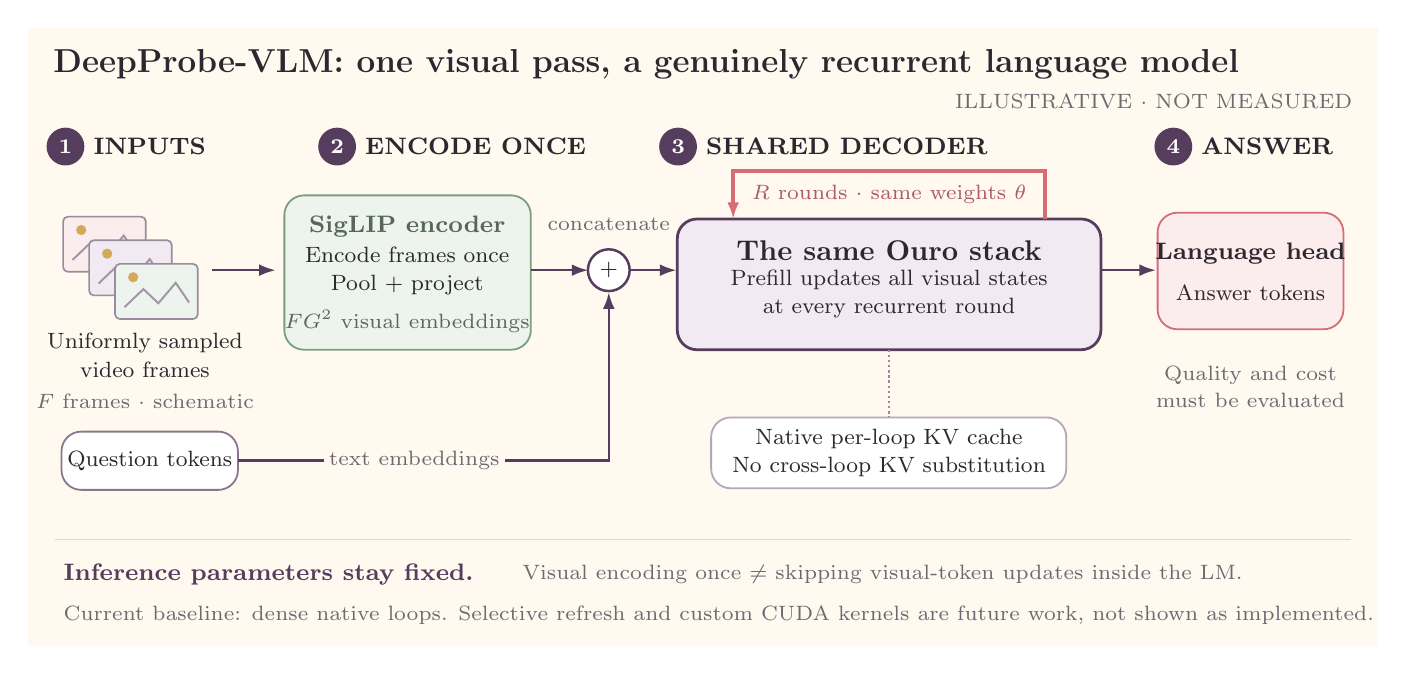
\begin{tikzpicture}[x=1cm,y=1cm]
\path[use as bounding box] (0,0) rectangle (17.145,7.85);
\fill[cream] (0,0) rectangle (17.145,7.85);
\node[title] at (.32,7.38) {DeepProbe-VLM: one visual pass, a genuinely recurrent language model};
\status{6.91}{muted}
% Four stages, one recurrence. Question tokens do not enter the vision tower.
\foreach \x/\n/\t in {.48/1/INPUTS,3.93/2/ENCODE ONCE,8.26/3/SHARED DECODER,14.55/4/ANSWER}{
  \node[circle,fill=aubergine,text=white,font=\bfseries\fontsize{7.6}{8}\selectfont,minimum size=4.8mm] at (\x,6.34) {\n};
  \node[label,anchor=west] at (\x+.35,6.34) {\t};
}
% Source frames are explicitly schematic, not empirical case studies.
\thumbnail{.45}{4.75}{blush}
\thumbnail{.78}{4.45}{lavender}
\thumbnail{1.11}{4.15}{mint}
\node[align=center] at (1.49,3.69) {Uniformly sampled\\video frames};
\node[sub] at (1.49,3.10) {$F$ frames $\cdot$ schematic};
\draw[flow] (2.34,4.77) -- (3.15,4.77);
% Visual encoder and deterministic pooling/projection.
\fill[card,fill=mint,draw=sage] (3.26,3.76) rectangle (6.39,5.72);
\node[label,text=sage!55!ink] at (4.82,5.32) {SigLIP encoder};
\node[align=center] at (4.82,4.76) {Encode frames once\\Pool + project};
\node[sub,text=sage!55!ink] at (4.82,4.12) {$F G^2$ visual embeddings};
\draw[flow] (6.39,4.77) -- (7.12,4.77);
% Merge is a token sequence, not another trainable router.
\node[circle,fill=white,draw=aubergine,line width=.9pt,minimum size=5.3mm] (join) at (7.38,4.77) {$+$};
\node[sub,align=center] at (7.38,5.35) {concatenate};
\draw[flow] (7.66,4.77) -- (8.24,4.77);
\fill[card,fill=white,draw=aubergine!70] (.43,1.98) rectangle (2.67,2.72);
\node[align=center] at (1.55,2.35) {Question tokens};
\draw[flow] (2.67,2.35) -- (7.38,2.35) -- (join.south);
\node[sub,fill=cream,inner sep=2pt] at (4.91,2.35) {text embeddings};
% True main-stack recurrence.
\fill[card,fill=lavender,draw=aubergine,line width=1pt] (8.25,3.76) rectangle (13.63,5.42);
\node[label,font=\bfseries\fontsize{10.3}{12}\selectfont] at (10.94,5.02) {The same Ouro stack};
\node[align=center] at (10.94,4.47) {Prefill updates all visual states\\at every recurrent round};
\draw[flow,draw=coral,line width=1.25pt] (12.92,5.42) -- (12.92,6.03) -- (8.96,6.03) -- (8.96,5.42);
\node[sub,text=coral!75!ink,fill=cream,inner sep=1pt] at (10.94,5.73) {$R$ rounds $\cdot$ same weights $\theta$};
\fill[card,fill=white,draw=aubergine!45] (8.68,2.00) rectangle (13.19,2.90);
\node[align=center] at (10.94,2.45) {Native per-loop KV cache\\No cross-loop KV substitution};
\draw[draw=aubergine!60,densely dotted,line width=.85pt] (10.94,3.76) -- (10.94,2.90);
% Model answer, no fabricated answer content.
\draw[flow] (13.63,4.77) -- (14.33,4.77);
\fill[card,fill=blush,draw=coral] (14.35,4.02) rectangle (16.71,5.50);
\node[label,align=center] at (15.53,4.98) {Language head};
\node[align=center] at (15.53,4.48) {Answer tokens};
\node[sub,align=center] at (15.53,3.29) {Quality and cost\\must be evaluated};
% One compact invariant strip instead of competing explanatory callouts.
\draw[line] (.35,1.35) -- (16.80,1.35);
\node[label,text=aubergine,anchor=west] at (.45,.91) {Inference parameters stay fixed.};
\node[sub,anchor=west] at (6.28,.91) {Visual encoding once $\neq$ skipping visual-token updates inside the LM.};
\node[sub,anchor=west] at (.45,.39) {Current baseline: dense native loops. Selective refresh and custom CUDA kernels are future work, not shown as implemented.};
\end{tikzpicture}
\end{document}
